\subsection{Proposed Solution}

wada wada

\subsubsection{Formal specification}
The formalisation and extension of the WAC specification will be
attained through subsequent refinement phases. In the tradition of
functorial semantics\cite{lawvere1963functorial, bonchi2017functorial},
a preliminary algebraic model will provide a concise, consistent and
unambiguous interpretation of WAC in terms of basic structures and
structure-preserving transformations in the elementary theory of the
categories of sets\cite{lawvere1964elementary, leinster2014rethinking}.
We will then engage with the WAC authors on GitHub to validate and
refine the model. Following that, we will devise a specification extension
to make the evaluation model more flexible so as to allow the evaluation
of access control policies expressed in terms of predicates on a generic
set---i.e., functions from a set $X$ to the Boolean algebra $\{0, 1\}$.
At the same time, we will investigate another specification extension
to accommodate data sharing through functional and homomorphic encryption
techniques. Finally, we will encode the formal specification in an
advanced programming language (either Haskell\cite{peytonjones:h98}
or Idris\cite{brady2013idris}) which we will then leverage to produce
a machine-checked proof of correctness of the resulting computer program.
The resulting (correct!) executable specification will be submitted to
the Solid project for consideration as a future version of WAC.

To illustrate our approach, consider WAC's authorisation process (\S 5)
and ACL resource discovery (\S 3.1). One possible interpretation of
the specification is that a server arranges information resources
in a tree $ResTree$ and, likewise, maintains an ACL resource tree
$ACLResTree$ containing the policies that protect the resources in
$ResTree$. Neither tree is empty. Now a tree is the same as a poset
with a terminal object. Each child-parent edge is a morphism
$child \rightarrow parent$ and the tree's root node is then terminal.

\begin{wrapfigure}{r}{0.5\textwidth}
  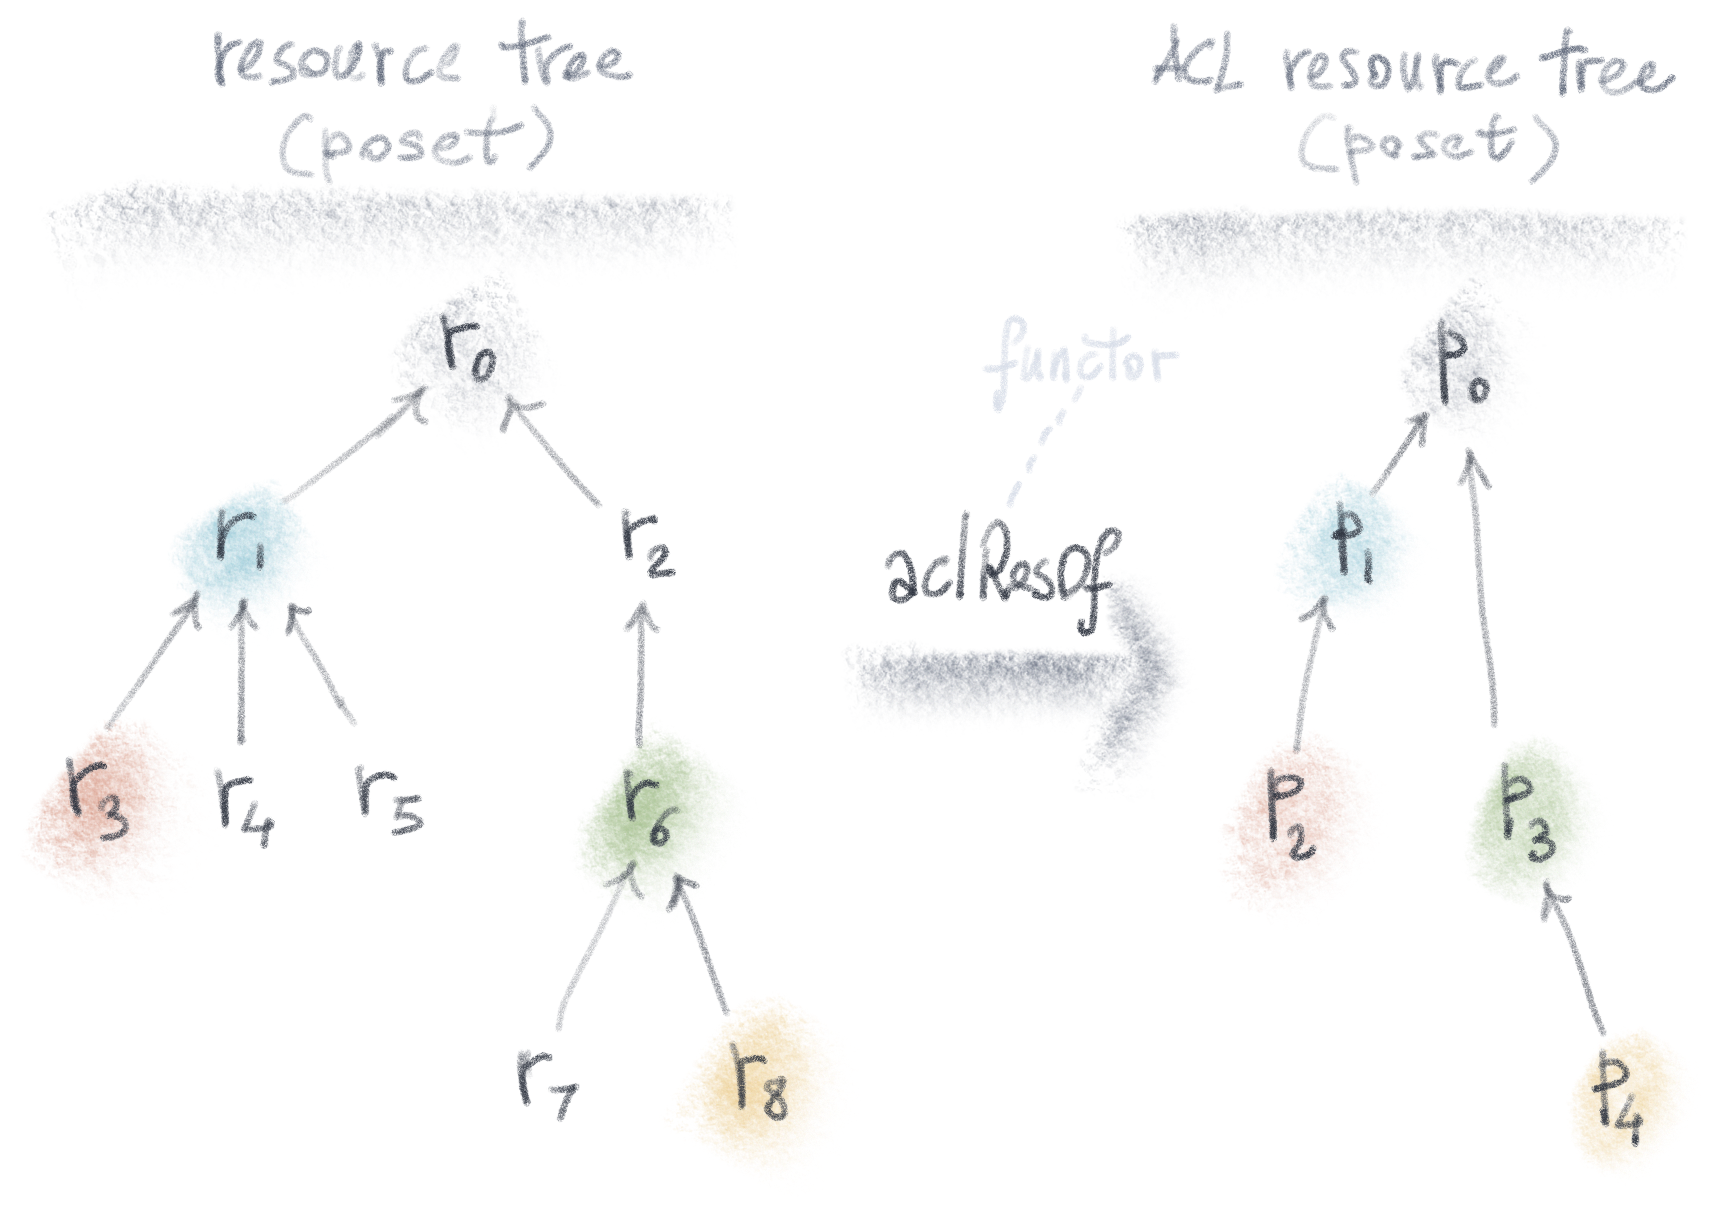
\includegraphics[width=0.5\textwidth]{effective-acl}
  % \caption{$aclResOf$ functor.}
  % \label{fig:aclResOf}
\end{wrapfigure}

On receiving an HTTP request, the server determines the ACL resource
that protects the resource which the request targets. This lookup
procedure is a functor $aclResOf : ResTree \rightarrow ACLResTree$.
Thus, each path $t_0 \rightarrow t_1 \rightarrow \ldots \rightarrow t_m$ in $ResTree$
goes to a path $u_0 \rightarrow u_1 \rightarrow \ldots \rightarrow u_n$
in $ACLResTree$ with $n \leq m$. Then if $r$ is the resource that
the incoming HTTP request targets, $aclResOf(r)$ is its corresponding
ACL resource. The figure on the right depicts an example $aclResOf$
functor. Colours hint how the functor maps resource nodes to ACL
resource nodes: $r_0$, $r_1$, $r_3$, $r_6$ and $r_8$ are mapped,
respectively, to $p_0$, $p_1$, $p_2$, $p_3$ and $p_4$. Since paths
must go to paths, $r_4$ and $r_5$ are forced to map to $p_1$. Ditto
for $r_7$ that must go to $p_3$. Finally, $r_2$ could either map to
$p_0$ or $p_3$, but in our example $aclResOf(r_2) = p_0$.

To translate an arbitrary $aclResOf$ functor into e.g. Haskell code,
observe that such a functor can be defined in terms of the function
$path$ which finds the path from the root of the tree to a node satisfying
a given predicate $p$. In turn, $path$ can easily be defined on a
canonical multi-way tree structure with the help of the standard
list processing function $concatMap$. It is just as easy to prove
$path$ correct by induction. Below is the corresponding Haskell code.
\\
\begin{lstlisting}[language=Haskell]
data Tree a = Node a [Tree a]

path :: (a -> Bool) -> Tree a -> [a]
path p = collect []
  where
  collect xs (Node a ts) | p a       = a:xs
                         | otherwise = concatMap (collect (a:xs)) ts
\end{lstlisting}


\subsubsection{Access control policies}
wada wada